\themaN
\graphicspath{{../Ch2_Nombres_entiers_et_decimaux/Images/}}

\chapter{Nombres entiers}
\label{C01}

%%%%%%%%%%%%%%%%%%%%%%%%%%%%%%%%%%%%%
\begin{prerequis}[Connaissances et compétences abordées]
   \begin{itemize}
      \item Connaître les unités de la numération décimale pour les nombres entiers (unités simples, dizaines, centaines, milliers, millions, milliards) et les relations qui les lient.
      \item Composer, décomposer les grands nombres entiers, en utilisant des regroupements par milliers.
      \item Comprendre et appliquer les règles de la numération décimale de position aux grands nombres entiers (jusqu’à 12 chiffres).
      \item Comparer, ranger, encadrer des grands nombres entiers, les repérer et les placer sur une demi-droite graduée adaptée.
   \end{itemize}
\end{prerequis}

\vfill

\begin{debat}[Débat : nombre ou chiffre ?]
   On croit souvent que les chiffres sont 0, 1, 2, 3, 4, 5, 6, 7, 8, 9 et que les nombres sont 10, 11, 12, 13, 14, 15, 16, 17, 18, 19, 20, 21\dots{} La vérité n'est pas si simple : un chiffre est un signe, un symbole, une forme pour représenter une quantité alors qu'un nombre désigne une quantité qui dépend d'une unité. Par exemple : \\ [5mm]
   \centerline{\textcolor{B1}{\fontsize{30}{30}\selectfont 8 \; - \; \fontsize{60}{60}\selectfont 5}} \\ [5mm]
   Le plus grand nombre est \og 8 \fg{} car il désigne la plus grande quantité alors que le plus grand chiffre est \og 5 \fg{} puisque c'est lui qui prend \og plus de place \fg.
   \bigskip
   \begin{cadre}[B2][F4]
      \begin{center}
         Vidéo : \href{https://www.youtube.com/watch?v=WRrLnktqUmE&feature=emb_logo}{\bf Raconte-moi une histoire : les petits cailloux}, chaîne YouTube {\it m@ths et tiques}, Yvan Monka.
      \end{center}
   \end{cadre}
\end{debat}

\vfill

\textcolor{PartieGeometrie}{\large\sffamily\bfseries Cahier de compétences} : chapitre 1, exercices 1, 18, 20, 21, 23, 37, 40, 41, 42. 


%%%%%%%%%%%%%%%%%%%%%%%%%%%%%%%%%%%%
%%%%%%%%%%%%%%%%%%%%%%%%%%%%%%%%%%%%%
\activites

\begin{activite}[Un abaque romain]
   {\bf Objectifs :} construire et utiliser un objet de calcul ancien ; comprendre et appliquer les règles de la numération décimale de position aux grands nombres entiers (jusqu’à 12 chiffres).
   \begin{QCM}
      \partie[construction de l'abaque]
         Un abaque est une table à calcul, le mot vient du latin {\it abax, abacus}. Il en existe de plusieurs formes. Celui que nous allons utiliser s'apparente à un abaque romain \og moderne \fg. \\
         Reproduire cet abaque sur une feuille de papier en mode paysage et au format A4 : sachant qu'il y a douze colonnes, quelle peut être la largeur d'une colonne ? \smallskip
         \begin{center}
         {\psset{unit=0.4}
         \begin{pspicture}(0,0)(36,16)
            \multido{\i=3+3}{11}{\psline(\i,0)(\i,14)}
            \multido{\i=0+9}{5}{\psline[linewidth=0.5mm](\i,0)(\i,16)}
            \psline[linewidth=0.5mm](0,16)(36,16)
            \psline[linewidth=0.5mm](0,12)(36,12)
            \textcolor{J1}{
               \rput(31.5,15){classe des unités}
               \rput(34.5,13){\texttt{I}}
               \rput(31.5,13){\texttt{X}}
               \rput(28.5,13){\texttt{C}}}
            \textcolor{B1}{
               \rput(22.3,15){classe des milliers}
               \rput(25.3,13){\texttt{I}}
               \rput(22.3,13){\texttt{X}}
               \rput(19.3,13){\texttt{C}}}
            \textcolor{A1}{
               \rput(13.1,15){classe des millions}
               \rput(16.1,13){\texttt{I}}
               \rput(13.1,13){\texttt{X}}
               \rput(10.1,13){\texttt{C}}}
            \rput(4,15){classe des milliards}
            \rput(7,13){\texttt{I}}
            \rput(4,13){\texttt{X}}
            \rput(1,13){\texttt{C}}
         \end{pspicture}}
         \end{center} \smallskip
      \partie[utilisation de l'abaque]
         Un abaque s'utilise traditionnellement avec des jetons, on peut utiliser par exemple des jetons de jeu, des cailloux, des grains, des petites pâtes\dots{}
         \begin{enumerate}
            \item Débattre de l'utilisation possible de l'abaque.
            \item Prendre un jeton et le placer dans l'une des colonnes de l'abaque. Quel nombre est représenté ? \\ [1mm]
               \pf \medskip
            \item Combien de nombres différents peut-on représenter avec un jeton ? Les lister. \\ [1mm]
               \pf \\ [3mm]
               \pf \medskip
            \item Combien de nombres différents peut-on représenter avec deux jetons ? En donner cinq. \\ [1mm]
               \pf \medskip
            \item Représenter les nombres suivants :
               \begin{colitemize}{3}
                  \item 123
                  \item mille-quatre-cent-quatre-vingts
                  \item 1\,023
                 \item deux-cent-trois-millions
                  \item 72\,105\,852
                  \item un-milliard-deux                        
               \end{colitemize}
            \item Quels sont les nombres représentés sur l'abaque au tableau ? \\ [1mm]
               \pf \bigskip
         \end{enumerate}
   \end{QCM}
 \end{activite}


%%%%%%%%%%%%%%%%%%%%%%%%%%%%%%%%%%%%%
\cours 

%%%%%%%%%%%%%%%%% %%%%%%%%%%%%%%%
\section{Écriture des nombres entiers}

Dans notre numération, il y a dix chiffres : 0, 1, 2, 3, 4, 5, 6, 7, 8 et 9. Avec ces chiffres, on peut écrire des nombres : il y en a une infinité et on les utilise avec des unités pour qu'ils aient un sens.

\begin{exemple*1}
   Une classe de 28 {\it élèves}, une voiture à 5 {\it places}, un sac de 20 {\it kg}, une pièce de 2 {\it euros}\dots
\end{exemple*1}


\begin{definition}
   Les nombres sont regroupés en classes composées de trois rangs : unités, dizaines, centaines.
   \begin{center}
      \begin{CLtableau}{\linewidth}{13}{c}
         \hline
         Classes & \multicolumn{3}{c|}{milliards} & \multicolumn{3}{c|}{millions} & \multicolumn{3}{c|}{milliers} & \multicolumn{3}{c|}{unités} \\
         \hline
         Valeurs & \rotatebox{90}{\;centaines\quad} & \rotatebox{90}{dizaines} & \rotatebox{90}{unités} &\rotatebox{90}{centaines} & \rotatebox{90}{dizaines} & \rotatebox{90}{unités} & \rotatebox{90}{centaines} & \rotatebox{90}{dizaines} & \rotatebox{90}{unités}  & \rotatebox{90}{centaines} & \rotatebox{90}{dizaines} & \rotatebox{90}{unités} \\
         \hline
         Exemple & & & & & 1 & 2 & 0 & 4 & 5 & 9 & 7 & 6 \\
         \hline
      \end{CLtableau} 
   \end{center}
\end{definition}

\begin{exemple*1}
   Dans le nombre 12\,045\,976 :
   \begin{colitemize}{2}
      \item 9 est le chiffre des centaines ;
      \item 5 est le chiffre des milliers ;
      \item 1 est le chiffre des dizaines de millions ;
      \item il y a 120\,459 centaines ;
      \item il y a 1\,204 dizaines de milliers ;
      \item il y a 12 millions.
   \end{colitemize}
\end{exemple*1}

On peut décomposer tout nombre sous sa forme canonique : \\
$\begin{array}{*{8}{l}}
   12\,045\,976 & =10\,000\,000 & + 2\,000\,000 & + 40\,000 & + 5\,000 & + 900 & + 70 & + 6 \\
      & =(1\times10\,000\,000) & + (2\times1\,000\,000) & + (4\times10\,000) & +(5\times1\,000) & +(9\times100) & +(7\times10) & +(6\times1) \\
      & =1\;\times10^7 & +\;2\times10^6 & +\;4\times10^4 & +\;5\times10^3 & +\;9\times10^2 & +\;7\times10^1 & +\;6\times10^0 \\
\end{array}$

La dernière écriture n'est pas au programme de la sixième : il s'agit de la décomposition du nombre dans la base 10 qui permet juste d'observer comment on écrit un nombre dans une base.

\begin{propriete}
   Règles orthographiques conformes à la réforme de 1990.
   \begin{itemize}
      \item Deux mots d'un même nombre sont séparés par un trait d'union ;
      \item {\it mille} est invariable ;
      \item {\it vingt} et {\it cent} prennent un \og s \fg{} lorsqu'il y en a plusieurs et qu'ils se trouvent à la fin ;
      \item {\it million} et {\it milliard} prennent toujours un \og s \fg{} quand il y en a plusieurs.
   \end{itemize}
\end{propriete}

\begin{exemple*1}
   \begin{itemize}
      \item 4\,000 : quatre-mille ;
      \item 80 : quatre-vingts et 81 : quatre-vingt-un ;
      \item 12\,045\,976 : douze-millions-quarante-cinq-mille-neuf-cent-soixante-seize.
    \end{itemize}
\end{exemple*1}


%%%%%%%%%%%%%%%%% III %%%%%%%%%%%%%%%
%%%%%%%%%%%%%%%%% III %%%%%%%%%%%%%%%
\section{La droite graduée}

\begin{definition}
   Pour graduer une droite, il faut choisir une {\bf origine} qui correspond au \og 0 \fg{} et une {\bf unité} qui sera reportée de manière régulière. \\
   Sur une droite graduée, un point est repéré par son {\bf abscisse}. \\
   \begin{pspicture}(-2,-1)(5.5,1)
   \psset{xunit=2}
      \psaxes[yAxis=false]{->}(0,0)(5.1,1)
      \psline[linecolor=violet]{<-}(-0.02,0.04)(-0.3,0.5)
      \rput(-0.6,0.5){\textcolor{violet}{origine}}
      \psline[linecolor=A1]{<->}(0,0.3)(1,0.3)
      \rput(0.5,0.6){\textcolor{A1}{unité}}
      \rput(3,0.4){\textcolor{B1}{A}}
      \psline[linecolor=B1]{<-}(3.02,0.04)(3.3,0.5)
      \rput(4.3,0.5){\textcolor{B1}{l'abscisse du point A est 3}}
   \end{pspicture}
\end{definition}
      
\begin{exemple*1}   
   \ \\
   \begin{pspicture}(-1,-0.5)(10,0.5)
      \psaxes[yAxis=false,labels=none]{->}(0,0)(10.5,0)
      \rput(0,-0.4){0}
      \rput(1,-0.4){100}
      \rput(3,0.4){A}
      \rput(7,0.4){R}
      \rput(10,0.4){C}
   \end{pspicture} \\
   Ici, l'unité vaut 100, donc les points A, R et C ont pour abscisses A(300), R(700) et C(1\,000).
\end{exemple*1}


%%%%%%%%%%%%%%%%%%%%%%%%%%%%%%%%%%
%%%%%%%%%%%%%%%%% III %%%%%%%%%%%%%%%
\section{Ordonner des nombres entiers}

\begin{definition}
   {\bf Comparer} deux nombres, c'est dire s'ils sont égaux ou si l'un est plus petit (ou plus grand) que l'autre.
\end{definition}

\begin{notation}
   le symbole \fbox{<} signifie \og plus petit que \fg{} et \fbox{>} signifie \og plus grand que \fg.
\end{notation}

\begin{exemple*1}
   $1\,000\,000\,200 > 1\,000\,000\,002$ \qquad ; \qquad $999\,999<1\,000\,000$.
\end{exemple*1}

\bigskip

\begin{definition}
   \begin{itemize}
      \item Ranger des nombres dans l'ordre {\bf croissant} signifie les ranger du plus petit au plus grand.
       \item Ranger des nombres dans l'ordre {\bf décroissant} signifie les ranger du plus grand au plus petit.
   \end{itemize}
\end{definition}

\begin{exemple*1}
   \begin{itemize}
      \item $1\,000\,045<1\,000\,085<1\,000\,600<1\,000\,607$ sont rangés dans l'ordre croissant.
      \item $321>312>231>213>132>123$ sont rangés dans l'ordre décroissant.
   \end{itemize}  
\end{exemple*1}

\begin{definition}
 {\bf Encadrer} un nombre, c'est l'entourer par un nombre plus petit et un nombre plus grand.
\end{definition}

\begin{exemple*1}
   On peut encadrer le nombre 8\,199 de différentes façons, par exemple :
   \begin{colitemize}{3}
     \item $8\,198<8\,199<8\,200$
     \item $8\,000<8\,199<9\,000$
     \item $1\,000<8\,199<10\,000$\dots
   \end{colitemize}
\end{exemple*1}


%%%%%%%%%%%%%%%%%%%%%%%%%%%%%%%%%%%%%%%
%%%%%%%%%%%%%%%%%%%%%%%%%%%%%%%%%%%%%%%
\exercicesbase

\begin{colonne*exercice}

\serie{Écrire des nombres entiers} %%%%%%%%%%%%%%%%%%%%

\begin{exercice} %1
   Écrire en chiffres les nombres suivants :
   \begin{enumerate}
      \item Sept-milliards-cinq-cent-cinquante-neuf-millions-deux-cent-quatre-vingt-huit-mille-trois-cents.
      \item Neuf-millions-sept-cent-mille-sept-cent-quarante. 
      \item Trente-huit-millions-trente-huit-mille.
      \item Vingt-six-milliards-cent-huit-millions-sept-cent-vingt-huit-mille-douze.
   \end{enumerate}
\end{exercice}

\bigskip

\begin{exercice} %1
   Écrire en lettres les nombres suivants :
   \begin{enumerate}
      \item 999.
      \item 58\,736.
      \item 53\,200\,000.
      \item 543\,823\,942\,900.
   \end{enumerate}
\end{exercice}

\bigskip

\begin{exercice}
   Voici cinq cartes contenant un nombre :
   \begin{center}
      \fbox{415} \qquad \fbox{2\,103} \qquad \fbox{9} \qquad \fbox{87} \qquad\fbox{13}
   \end{center}
   Placer ces cartes côte à côte pour écrire :
   \begin{enumerate}
      \item le plus petit nombre entier de douze chiffres ;
      \item le plus grand nombre entier.
   \end{enumerate}
\end{exercice}

\bigskip

\begin{exercice}
   Dans le nombre 6\,083\,472 donner :
   \begin{enumerate}
      \item le chiffre des unités ;
      \item le chiffre des dizaines de mille ;
      \item le chiffre des unités de millions ;
      \item le nombre de centaines ;
      \item le nombre de centaines de mille ;
      \item le nombre de millions.
   \end{enumerate}
\end{exercice}

\bigskip

\begin{exercice}
   Écrire en chiffres chacun des nombres.
   \begin{enumerate}
      \item 13 centaines et 25 unités.
      \item 43 millions et 8 dizaines.
      \item 25 dizaines de mille et 67 centaines.
      \item 12 dizaines de milliards et 3 centaines de millions.
   \end{enumerate}
\end{exercice}

\bigskip

\begin{exercice}
  Écrire le résultat des opérations :
   \begin{enumerate}
      \item $(1\times1\,000) + (4\times100) + (8\times10)$
      \item $(3\times100\,000) + (6\times10\,000) + (1\times10)$
      \item $(2\times1\,000\,000) + (9\times1\,000) + (5\times1)$
      \item $(7\times1\,000\,000\,000) + (7\times1\,000) + (3\times100)$
   \end{enumerate}
\end{exercice}


\serie{Ordonner des nombres entiers} %%%%%%%%%%%%%%%%%%%

\begin{exercice}
   Écrire l'abscisse de chacun des points représentés sur la droite graduée.
   \begin{enumerate}
   \small
      \item \begin{pspicture}(0,0)(8,0.7)
                  \psset{xunit=5}
                  \psaxes[yAxis=false,subticks=10,subtickcolor=gray]{->}(0,0)(1.5,0)
                  \pstGeonode[PosAngle=90](0.3,0){A}(0.8,0){B}(1.1,0){C}(1.3,0){D}
                  \rput(1.024,-0.415){0}
               \end{pspicture}
      \item \begin{pspicture}(0,0)(8,1.2)
                  \psset{xunit=1.15}
                  \psaxes[yAxis=false,subticks=2,subtickcolor=gray,labels=none]{->}(0,0)(6.5,0)
                  \rput(1,-0.4){1\,000}
                  \rput(2,-0.4){2\,000}
                  \pstGeonode[PosAngle=90](1.5,0){J}(3.5,0){K}(5.5,0){L}
               \end{pspicture}
      \item \begin{pspicture}(0,0)(8,1.2)
                  \psset{xunit=0.47}
                  \psline{->}(0,0)(16,0)
                  \multido{\n=0+1}{15}{\psline[linecolor=gray,linewidth=0.1mm](\n,-0.1)(\n,0.1)}
                  \psline(3,-0.1)(3,0.1)
                  \rput(3,-0.4){29\,000}
                  \psline(13,-0.1)(13,0.1)
                  \rput(13,-0.4){30\,000}
                  \pstGeonode[PosAngle=90](2,0){R}(7,0){S}(10,0){T}(14,0){U}
               \end{pspicture}
   \end{enumerate}
\end{exercice}

\ \\

\begin{exercice}
   Placer les points dont l'abscisse est donnée sur les droites graduées. \smallskip
   \begin{enumerate}
   \small
      \item E(121) \qquad F(123) \qquad G(125) \qquad H(131) \\
         \begin{pspicture}(0,-0.8)(8,0.7)
                  \psset{xunit=5}
                  \psaxes[yAxis=false,Ox=120,dx=1,Dx=10,subticks=10,subtickcolor=gray]{->}(0.2,0)(1.5,0)
                  \psline(0,0)(0.2,0)
                  \psline[linewidth=0.07mm](0.1,0.1)(0.1,-0.1)
               \end{pspicture} 
      \item M(7\,810) \qquad N(7\,830) \qquad P(7\,890) \qquad Q(7\,910) \\
         \begin{pspicture}(0,-0.8)(8,0.7)
                  \psset{xunit=0.45}
                  \psline{->}(0,0)(16,0)
                  \multido{\n=0+1}{16}{\psline[linecolor=gray,linewidth=0.1mm](\n,-0.1)(\n,0.1)}
                  \psline(2,-0.1)(2,0.1)
                  \rput(2,-0.4){7\,800}
                  \psline(12,-0.1)(12,0.1)
                  \rput(12,-0.4){7\,900}
               \end{pspicture}
       \item V(640\,800) \qquad W(641\,300) \qquad Y(641\,600) \qquad Z(641\,800) \\
          \begin{pspicture}(0,-0.5)(8,0.7)
                  \psset{xunit=0.45}
                  \psline{->}(0,0)(16,0)
                  \multido{\n=0+1}{16}{\psline[linecolor=gray,linewidth=0.1mm](\n,-0.1)(\n,0.1)}
                  \psline(4,-0.1)(4,0.1)
                  \rput(4,-0.4){641\,000}
                  \psline(14,-0.1)(14,0.1)
                  \rput(14,-0.4){642\,000}
               \end{pspicture}
   \end{enumerate}
\end{exercice}

\bigskip

\begin{exercice}
   Ranger chaque série de nombres :
   \begin{enumerate}
      \item dans l'ordre croissant. \\ [1mm]
         \fbox{1\,110} \; \fbox{1\,101} \; \fbox{1\,011} \; \fbox{1\,111} \; \fbox{1\,100} \; \fbox{1\,010} \smallskip
      \item dans l'ordre décroissant. \\ [1mm]
         \fbox{128} \; \fbox{182} \; \fbox{281} \; \fbox{218} \; \fbox{280} \; \fbox{821} \; \fbox{812}
   \end{enumerate}
\end{exercice}

\bigskip

\begin{exercice}
   Encadrer avec l'entier précédent et suivant. \medskip
   \begin{enumerate}
      \item \pfh < 850 < \pfh\mbox{} \medskip
      \item \pfh < 9\,901 < \pfh\mbox{} \medskip
      \item \pfh < 956 < \pfh\mbox{} \medskip
      \item \pfh < 29\,008 < \pfh\mbox{} \medskip
      \item \pfh < 12\,309 < \pfh\mbox{} \medskip
      \item \pfh < 77\,777 < \pfh\mbox{}
   \end{enumerate}
\end{exercice}

\end{colonne*exercice}


%%%%%%%%%%%%%%%%%%%%%%%%%%%%%%%%%%%%%%%
%%%%%%%%%%%%%%%%%%%%%%%%%%%%%%%%%%%%%%%
\Recreation

\enigme[La numération égyptienne]
   \partie[introduction]
      L'Égypte antique est une ancienne civilisation qui a vécu un peu plus de $3000$ ans entre $3150$ av. J.-C. et $30$ av. J.-C., elle s'est développée le long du Nil. Les Égyptiens maitrisent l'écriture, ils utilisent des symboles qui représentent des choses réelles ou non grâce à des hiéroglyphes. \\ [3mm]
      \begin{minipage}{6.5cm}
         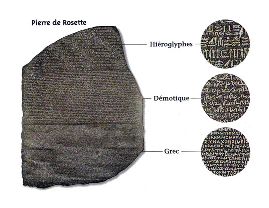
\includegraphics[width=6cm]{rosette}
      \end{minipage}
      \qquad
      \begin{minipage}{9.5cm}
         En 1821, Jean-François Champollion réussit à décrypter les caractères égyptiens. Comment a-t-il pu réussir cet exploit ? On pourra s'aider de l'image ci-contre. \\ [3mm]
         \pf \\ [3mm]
         \pf \\ [3mm]
         \pf
      \end{minipage}

      \bigskip
      
   \partie[la numération égyptienne]
      \begin{enumerate}
         \item Dans la numération égyptienne, voilà comment on écrit certains nombres indo-arabes : \smallskip
         \begin{center} 
            \begin{tabular}{|c|c|c|c|c|}
               \hline
               18 & 70 & 235 & 3\,018 & 1\,230\,012 \\
               \hline
               & & & & \\ [-3mm]
               \Large\textpmhg{\Hten\Hone\Hone\Hone\Hone\Hone\Hone\Hone\Hone}
               &
               \Large\textpmhg{\Hten\Hten\Hten\Hten\Hten\Hten\Hten}
               & 
               \Large\textpmhg{\Hhundred\Hhundred\Hten\Hten\Hten\Hone\Hone\Hone\Hone\Hone} & \Large\textpmhg{\Hthousand\Hthousand\Hthousand\Hten\Hone\Hone\Hone\Hone\Hone\Hone\Hone\Hone}
               &
               \Large\textpmhg{\Hmillion\HCthousand\HCthousand\HXthousand\HXthousand\HXthousand\Hten\Hone\Hone} \\
               \hline
            \end{tabular}
         \end{center} \medskip
      À la manière de Champollion, retrouver la valeur de ces symboles égyptiens. \smallskip
      \begin{center}
         \begin{tabular}{|C{1.8}|C{1.8}|C{1.8}|C{1.8}|C{1.8}|C{1.8}|C{1.8}|}
            \hline
            & & & & & & \\ [-3mm]
            \Large\textpmhg{\Hone}
            &
            \Large\textpmhg{\Hten}
            &
            \Large\textpmhg{\Hhundred}
            &
            \Large\textpmhg{\Hthousand}
            &
            \Large\textpmhg{\HXthousand}
            &
            \Large\textpmhg{\HCthousand}
            &
            \Large\textpmhg{\Hmillion} \\
            \hline
            & & & & & & \\ [3mm]
           \hline
         \end{tabular}
      \end{center}
 
      \bigskip
   
      \item Écrire les nombres égyptiens suivants en nombres indo-arabes : \\ [2mm]
      {\Large\textpmhg{\HXthousand\Hthousand\Hthousand\Hten\Hten\Hten\Hten\Hten\Hten}} : \pf \\ [3mm]
      {\Large\textpmhg{\HCthousand\HXthousand\HXthousand\HXthousand\Hthousand\Hthousand\Hthousand\Hhundred\Hhundred\Hhundred\Hten\Hten\Hten\Hten\Hone\Hone\Hone\Hone\Hone\Hone\Hone\Hone}} : \pf \\  [3mm]
      {\Large\textpmhg{\Hmillion\Hmillion\Hmillion\HCthousand\Hone\Hone}} : \pf \\
      \item Écrire les nombres indo-arabes suivants en nombres égyptiens : \\ [4mm]
      8\,032 : \pf \\ [5mm]
      3\,000\,100 :  \pf \\
      \item Quel nombre présent dans notre numération écrite n'existe pas dans la numération égyptienne ? Pourquoi ? \\ [3mm]
      \pf
      \end{enumerate}

